\documentclass[conference]{IEEEtran}

\usepackage[T1]{fontenc}
\usepackage[utf8]{inputenc}
\usepackage{amsmath}
\usepackage{graphicx}
\usepackage{booktabs}
\usepackage{hyperref}
\usepackage{microtype}
\usepackage{cite}
\usepackage{placeins}

\hypersetup{colorlinks=true, linkcolor=black, citecolor=black, urlcolor=black}
\setlength{\textfloatsep}{8pt plus 1pt minus 2pt}
\setlength{\floatsep}{8pt plus 1pt minus 2pt}
\setlength{\intextsep}{8pt plus 1pt minus 2pt}

\begin{document}

\title{Does the Order of Training Data Influence Optimization?}

\author{
\IEEEauthorblockN{Niels Enkaoua, R\'emi Germi, Mohamed Sami Ghrab}
\IEEEauthorblockA{EPFL\\Optimization for Machine Learning Mini-Project, Spring 2026}
}

\maketitle

\begin{abstract}
We study how training-data order changes stochastic gradient descent when
the dataset, model, and hyperparameters are fixed.
Using Fashion-MNIST, a small CNN, momentum SGD, 10 epochs, and seeds 0, 1,
and 2, we compare two IID orders, two curricula, and two label-based
non-IID streams.
Random reshuffling gives the best final accuracy
($89.47\pm0.68\%$), fixed random order is slightly worse, and
hard-to-easy curriculum clearly outperforms easy-to-hard.
The two label-based orders collapse to chance accuracy at the reference
learning rate.
The recorded diagnostics show why: sorted label streams create
highly aligned or non-finite update sequences, degenerate single-class
predictors, and a much narrower stability region.
Lowering the learning rate partially rescues training but not balanced
generalization.
Two further controls show the failure is general but its severity is not:
AdamW partially rescues class-blocked streams yet keeps a narrow stability
region, while a convex logistic-regression model degrades under the same
orders but never collapses to chance.
Data order therefore changes both SGD stability and the quality of the
final classifier, and its catastrophic mode is specific to non-convex
training.
\end{abstract}

\section{Introduction}
Mini-batch SGD is usually analyzed under an approximately IID sampling
assumption, which random reshuffling approximates in practice
\cite{bottou2018,gurbuzbalaban2021}.
If the training stream becomes structured, however, consecutive updates
need not explore diverse directions: momentum can instead accumulate a
persistent bias.
We test that mechanism directly by varying only the order of
Fashion-MNIST examples while keeping the model, optimizer, and data split
fixed.
The central question is whether ordering changes both optimization
stability and the final multi-class classifier.

Prior work establishes \emph{why} random reshuffling outperforms
with-replacement sampling theoretically \cite{gurbuzbalaban2021} and
studies hand-designed curricula \cite{bengio2009curriculum}; our
experiments add the complementary empirical view: how badly, and through
which mechanism, optimization fails when the IID assumption is broken,
and whether that failure depends on the optimizer (SGD vs.\ AdamW
\cite{loshchilov2019adamw}) and on the model class (non-convex CNN vs.\
convex logistic regression).

\section{Experimental Setup}
We train a compact CNN on Fashion-MNIST \cite{xiao2017fashion} with SGD,
momentum $0.9$, weight decay $5\times10^{-4}$, batch size $128$, and
reference learning rate $0.05$.
All main runs use 10 epochs, seeds 0, 1, and 2, and a stratified subset
of 20{,}000 training examples.
We compare \texttt{random}, \texttt{fixed\_random},
\texttt{curriculum\_easy}, \texttt{curriculum\_hard},
\texttt{label\_sorted}, and \texttt{label\_block\_random}.
For each run we record epoch-wise accuracy and loss, gradient cosine
similarity between consecutive steps, per-class test accuracy, forgetting,
and final prediction distributions.
Two control studies repeat key orderings with AdamW (learning rates
$10^{-3}$ and $10^{-2}$) and with a convex logistic-regression model
(SGD, learning rate $0.05$).

\begin{table}[!t]
  \centering
  \caption{Training-data orders used in the study.}
  \label{tab:orders}
  \begin{tabular}{@{}p{0.35\columnwidth}p{0.57\columnwidth}@{}}
    \toprule
    Ordering & Construction rule \\
    \midrule
    \texttt{random} & Fresh random permutation at every epoch. \\
    \texttt{fixed\_random} & One random permutation reused for all epochs. \\
    \texttt{curriculum\_easy} & Samples sorted from easy to hard once, then reused. \\
    \texttt{curriculum\_hard} & Samples sorted from hard to easy once, then reused. \\
    \texttt{label\_sorted} & Samples fully grouped by class label in a fixed order. \\
    \texttt{label\_block\_random} & Class-homogeneous blocks with reshuffled block order across epochs. \\
    \bottomrule
  \end{tabular}
\end{table}
\FloatBarrier

\section{Results}
\subsection{Global Results}
Figure~\ref{fig:global-accuracy} shows the overall ranking.
Random reshuffling is the strongest baseline at
$89.47\pm0.68\%$, followed by fixed random order at
$88.46\pm0.49\%$.
Among deterministic non-IID schedules, hard-to-easy curriculum reaches
$84.53\pm0.93\%$ and clearly dominates easy-to-hard at
$70.71\pm2.74\%$.
The two label-based orders collapse to exactly $10\%$ test accuracy,
which is chance level for this balanced ten-class task.
The main qualitative split is therefore between trainable orders
(\texttt{random}, \texttt{fixed\_random}, and both curricula) and
class-separated streams, which fail completely at the reference step size.

\begin{figure}[t]
  \centering
  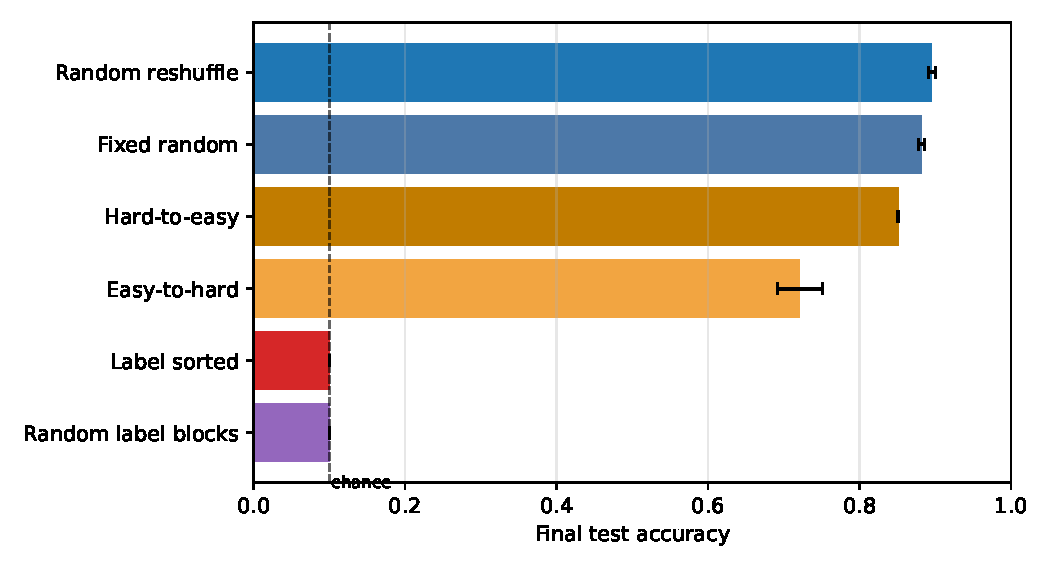
\includegraphics[width=\columnwidth]{results_v8/figures/global_final_accuracy.pdf}
  \caption{Final test accuracy at learning rate $0.05$.
  Error bars show one standard deviation across seeds 0, 1, and 2.
  Random reshuffling is best; both label-based orders collapse to chance.}
  \label{fig:global-accuracy}
\end{figure}

\begin{figure}[!t]
  \centering
  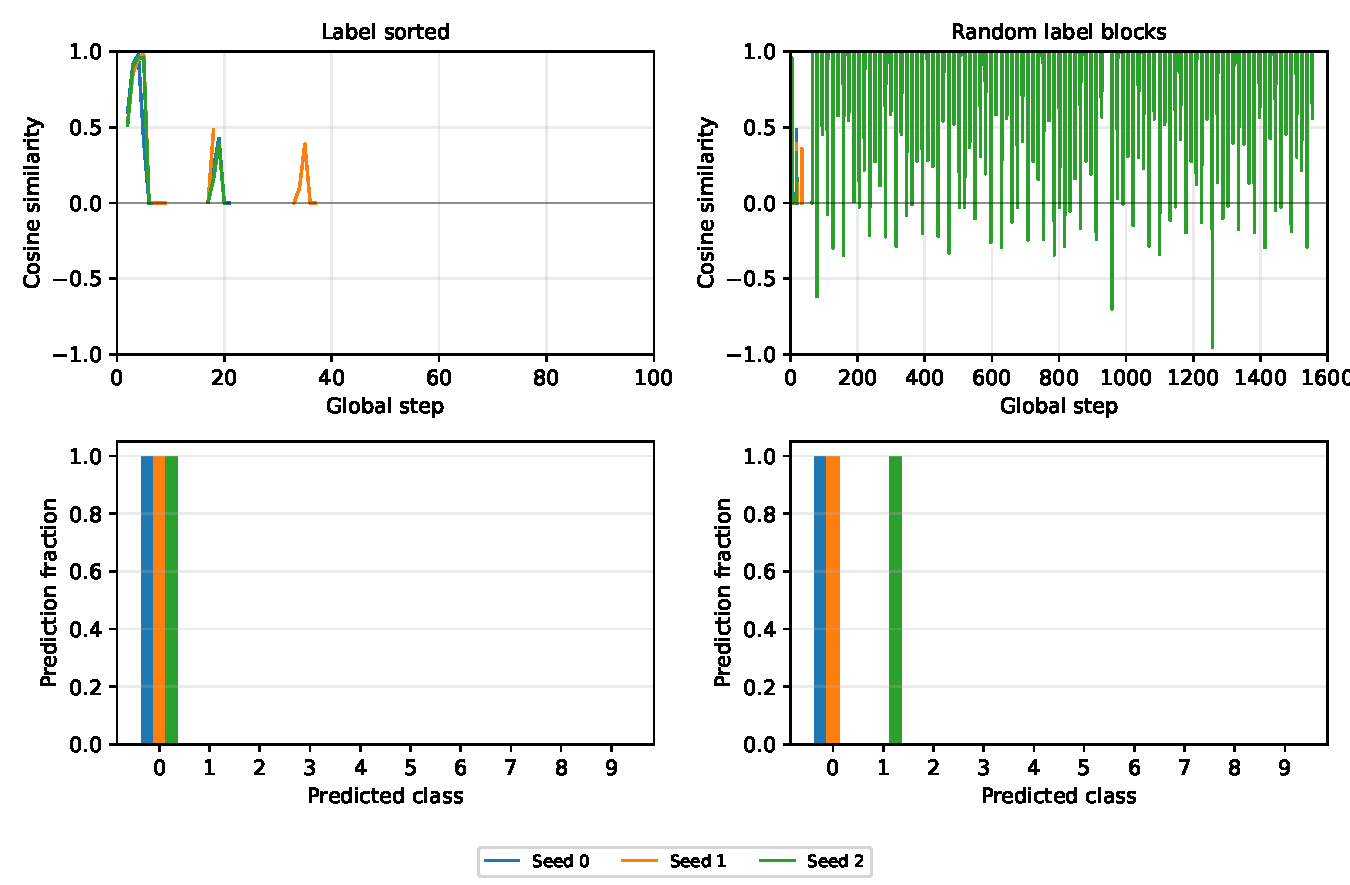
\includegraphics[width=\columnwidth]{results_v8/figures/failure_overview.pdf}
  \caption{Failure diagnostics at learning rate $0.05$ for the two
  pathological orders.
  Top row: gradient cosine similarity per seed; lines terminate when
  finite values disappear.
  Bottom row: final predicted-class distributions per seed.
  \texttt{label\_sorted} collapses identically across seeds, whereas
  \texttt{label\_block\_random} is seed-dependent numerically but still
  converges to single-class predictors.}
  \label{fig:failure-overview}
\end{figure}

\subsection{Failure Analysis of Label-Based Orders}
The failure modes are not just low-accuracy outcomes; they are unstable
optimization trajectories.
Figure~\ref{fig:failure-overview} shows that \texttt{label\_sorted}
predicts class 0 for every test image in all three seeds, while
\texttt{label\_block\_random} collapses to class 0 for seeds 0 and 1 and
to class 1 for seed 2.
The cosine traces reveal why.
For \texttt{label\_sorted}, only 13, 18, and 11 finite step-to-step
gradient cosines remain for seeds 0, 1, and 2, with last finite steps 64,
80, and 48 out of 1570 total pairs.
For \texttt{label\_block\_random}, seeds 0 and 1 fail almost
immediately (19 and 48 finite steps), while seed 2 stays finite to the
end but still converges to a degenerate one-class predictor.
This seed-dependent split shows that blockwise label order is numerically
less brittle than fully sorted order, yet just as poor functionally.

Appendix~\ref{app:lr} shows the same pattern across epochs and learning
rates.
At $0.05$ and $0.1$, both label-based orders remain at
$10.00\pm0.00\%$.
Lowering the learning rate to $0.001$ partially rescues optimization,
raising \texttt{label\_sorted} to $31.95\pm8.42\%$ and
\texttt{label\_block\_random} to $40.00\pm5.94\%$.
However, the rescue is incomplete and still structurally biased:
the dominant predicted class keeps 36--53\% of the test set for
\texttt{label\_sorted} and 30--40\% for
\texttt{label\_block\_random}, with only five to seven classes receiving
any predictions.
Thus a smaller step size softens collapse but does not restore balanced
multi-class learning.
Appendix~\ref{app:failure} confirms this at the class level and is
consistent with catastrophic forgetting under sequentially biased streams
\cite{mccloskey1989}.

\subsection{Stable Methods}
The four trainable orders remain finite for essentially the whole run:
each keeps valid gradient-cosine values on more than $99.9\%$ of recorded
step pairs.
The two IID baselines also have the weakest directional alignment, with
mean cosine similarity $0.200$ for \texttt{random} and $0.201$ for
\texttt{fixed\_random}.
The curriculum variants are more correlated
($0.249$ for \texttt{curriculum\_easy}, $0.259$ for
\texttt{curriculum\_hard}), which is consistent with their lower final
accuracy and with the idea that deterministic structure reduces gradient
diversity even when it does not cause outright collapse.

The stable methods differ mainly in class balance and retention.
Appendix~\ref{app:stable} shows that \texttt{random} and
\texttt{fixed\_random} keep the most even class-wise behavior: at epoch 10,
their weakest-class accuracies are 0.680 and 0.667, respectively.
For \texttt{curriculum\_hard}, the weakest class remains much lower at
0.447, but this is still substantially better than
\texttt{curriculum\_easy}, whose weakest class reaches only 0.273.
The forgetting diagnostic tells the same story.
Final mean forgetting is small for \texttt{random} (0.0467),
\texttt{fixed\_random} (0.0427), and \texttt{curriculum\_hard} (0.0253),
but rises to 0.123 for \texttt{curriculum\_easy}.
Among deterministic curricula, the order of difficulty therefore matters:
hard-to-easy remains clearly more stable and better balanced than
easy-to-hard.

\subsection{Robustness Across Optimizers and Model Classes}
\label{sec:robustness}
Two control studies test whether the ordering effects above are specific
to momentum SGD on a non-convex model (Table~\ref{tab:robustness}).
First, AdamW at its standard learning rate $10^{-3}$ reproduces the
ordering hierarchy and \emph{partially} rescues the class-blocked stream:
\texttt{label\_block\_random} reaches $40.6\pm13.3\%$ instead of
collapsing to $10\%$ as under SGD at the reference step size, suggesting
that adaptive per-coordinate step sizes dampen the bias accumulated over
class-homogeneous updates.
The rescue is fragile: at learning rate $10^{-2}$, AdamW collapses to
chance not only on \texttt{label\_block\_random} but also on
\texttt{curriculum\_hard}, which SGD trains without difficulty, and
\texttt{fixed\_random} becomes seed-dependent ($61.1\pm44.2\%$).
The narrow stability region under structured streams is therefore not an
artifact of SGD; for the adaptive optimizer it is, if anything, narrower.
Second, the convex logistic-regression model never collapses: its worst
order (\texttt{label\_sorted}, $52.9\%$) stays far above chance, although
ordering still costs up to 28 accuracy points relative to random
reshuffling ($80.9\pm0.3\%$).
The catastrophic single-class failure mode therefore requires
non-convexity; on a convex objective, structured orders merely slow and
bias optimization, in line with incremental-gradient theory
\cite{bottou2018,gurbuzbalaban2021}.

\begin{table}[!t]
  \centering
  \caption{Final test accuracy (\%, mean $\pm$ std over seeds 0--2) for the
  optimizer and model-class controls. CNN/SGD at the reference learning
  rate $0.05$ is the main experiment (Fig.~\ref{fig:global-accuracy}).
  Dashes denote orderings not included in the control runs.}
  \label{tab:robustness}
  \begin{tabular}{@{}lccc@{}}
    \toprule
    & \multicolumn{2}{c}{CNN, AdamW} & Logistic, SGD \\
    \cmidrule(lr){2-3} \cmidrule(l){4-4}
    Ordering & lr $10^{-3}$ & lr $10^{-2}$ & lr $0.05$ \\
    \midrule
    \texttt{random}             & $89.6\pm0.4$  & $87.1\pm0.8$   & $80.9\pm0.3$ \\
    \texttt{fixed\_random}      & $88.6\pm0.2$  & $61.1\pm44.2$  & $81.0\pm1.6$ \\
    \texttt{curriculum\_easy}   & --            & --             & $58.4\pm0.8$ \\
    \texttt{curriculum\_hard}   & $86.3\pm0.3$  & $10.0\pm0.0$   & $79.0\pm0.0$ \\
    \texttt{label\_sorted}      & --            & --             & $52.9\pm0.0$ \\
    \texttt{label\_block\_random} & $40.6\pm13.3$ & $10.0\pm0.0$ & $58.0\pm11.1$ \\
    \bottomrule
  \end{tabular}
\end{table}
\FloatBarrier

\section{Conclusion}
Data order changes SGD in a mechanically meaningful way.
Random reshuffling gives the best and most robust behavior, fixed random
order is consistently weaker, and curriculum design matters even when the
stream remains trainable.
The strongest effect appears for class-separated streams, which produce
degenerate single-class predictors, non-finite gradient diagnostics, and a
much narrower learning-rate stability region.
Lowering the step size helps, but it does not remove the structural bias
introduced by non-IID ordering.
The control studies sharpen this picture: adaptive step sizes (AdamW)
mitigate but do not repair the damage, and a convex model degrades
gracefully where the CNN collapses, identifying the catastrophic mode as
a genuinely non-convex phenomenon.
In this controlled setting, data order is therefore not a benign
implementation detail but a direct control knob on optimization stability
and generalization.

\paragraph{Reproducibility}
The main 10-epoch outputs are produced by
\texttt{python run\_v3.py} (directories \texttt{results\_v3\_main} and
\texttt{results\_v3\_lr0p1}) together with
\texttt{python run.py -{}-epochs 10 -{}-seeds 0 1 2
-{}-max-train-examples 20000 -{}-orders label\_sorted
label\_block\_random -{}-lr 0.001 -{}-output-dir results\_lr0001}.
The optimizer and model-class controls of
Section~\ref{sec:robustness} are produced by
\texttt{python run\_v3.py -{}-skip-main -{}-skip-sweep
-{}-compare-adamw -{}-compare-logistic} (directories \texttt{results\_adamw\_lr0p001},
\texttt{results\_adamw\_lr0p01}, and
\texttt{results\_logistic\_comparison}; Table~\ref{tab:robustness} reports
their \texttt{tables/final\_test\_accuracy.csv}).
All report figures are rebuilt from the stored outputs with
\texttt{python build\_report\_v8\_assets.py}; no experiments are rerun.

\appendices
\section{Additional Accuracy and Learning-Rate Curves}
\label{app:lr}
This appendix reports the epoch-wise accuracy trajectories for all six
orders and the learning-rate sensitivity of the two failing orders
(Figs.~\ref{fig:app-trajectories} and~\ref{fig:app-lr}).

\begin{figure}[!h]
  \centering
  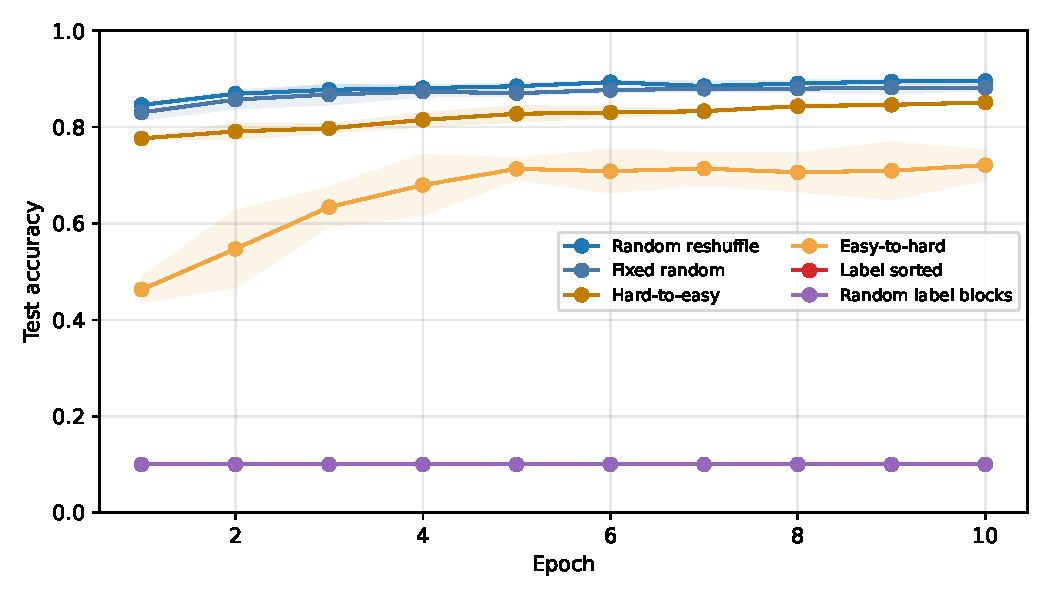
\includegraphics[width=\columnwidth]{results_v8/figures/global_accuracy_trajectories.pdf}
  \caption{Test-accuracy trajectories for all six orders at the reference
  learning rate $0.05$. The two label-based orders collapse from the first
  epoch.}
  \label{fig:app-trajectories}
\end{figure}

\begin{figure}[!h]
  \centering
  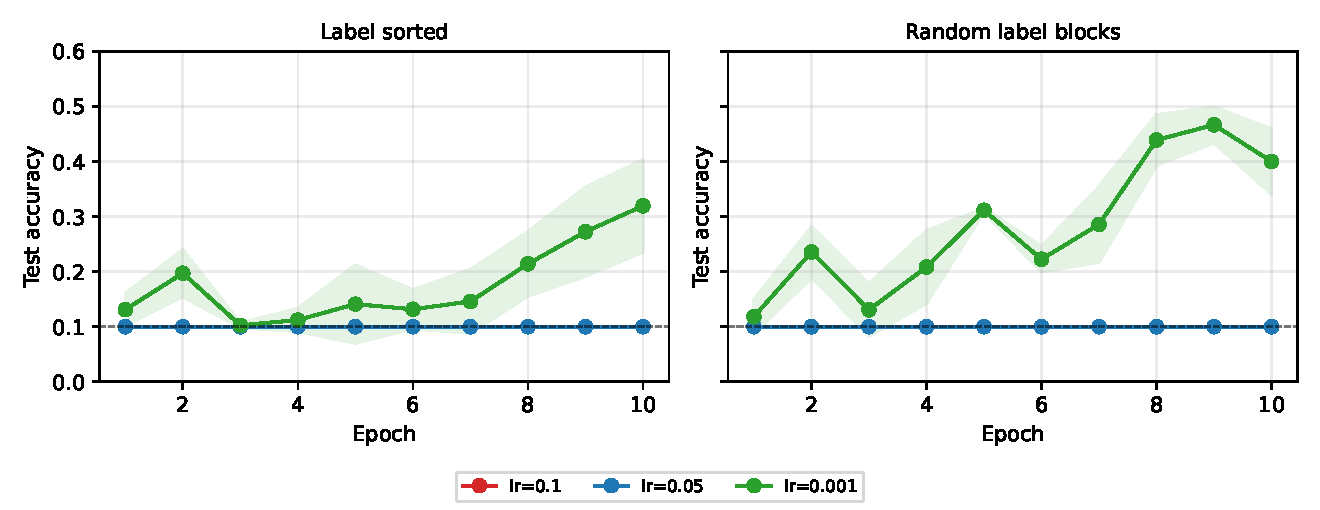
\includegraphics[width=\columnwidth]{results_v8/figures/failure_lr_trajectories.pdf}
  \caption{Learning-rate sensitivity of the failing orders.
  Lowering the learning rate to $0.001$ partially rescues test accuracy but
  does not approach the reshuffled baseline.}
  \label{fig:app-lr}
\end{figure}
\FloatBarrier

\section{Label-Order Class Diagnostics}
\label{app:failure}
This appendix shows the per-class accuracy evolution of the two
label-based orders (Fig.~\ref{fig:app-heatmaps}): the models specialize to
a narrow class subset rather than learning a balanced classifier.

\begin{figure}[!h]
  \centering
  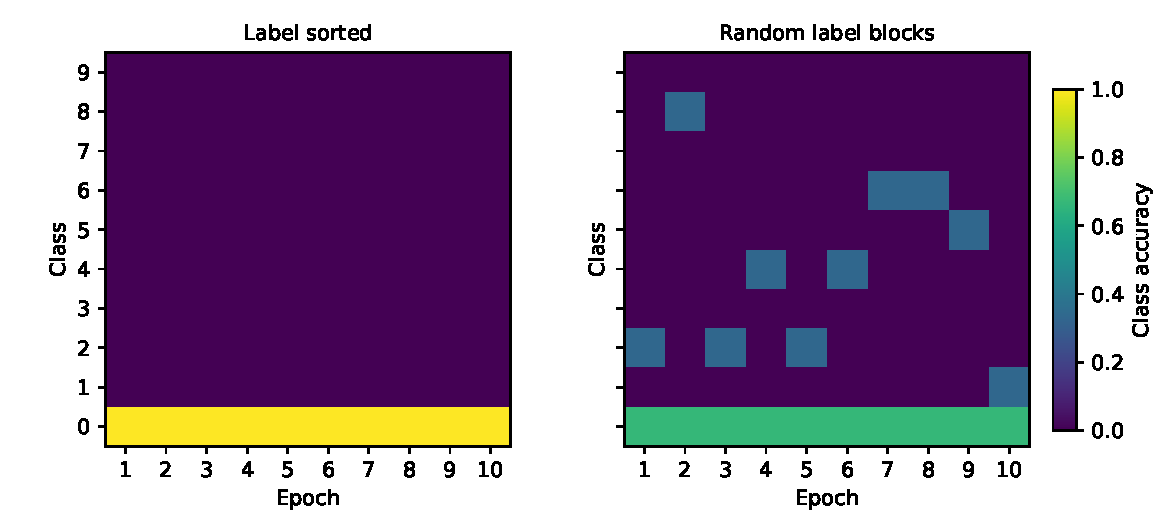
\includegraphics[width=\columnwidth]{results_v8/figures/failure_class_heatmaps.pdf}
  \caption{Per-class test accuracy across epochs for the two label-based
  orders at learning rate $0.05$.
  The models specialize to a narrow class subset rather than learning a
  balanced classifier.}
  \label{fig:app-heatmaps}
\end{figure}
\FloatBarrier

\section{Stable-Method Diagnostics}
\label{app:stable}
This appendix collects the gradient-alignment, class-balance, and
forgetting diagnostics for the four trainable orders
(Figs.~\ref{fig:app-cosine}--\ref{fig:app-forgetting}).

\begin{figure*}[!h]
  \centering
  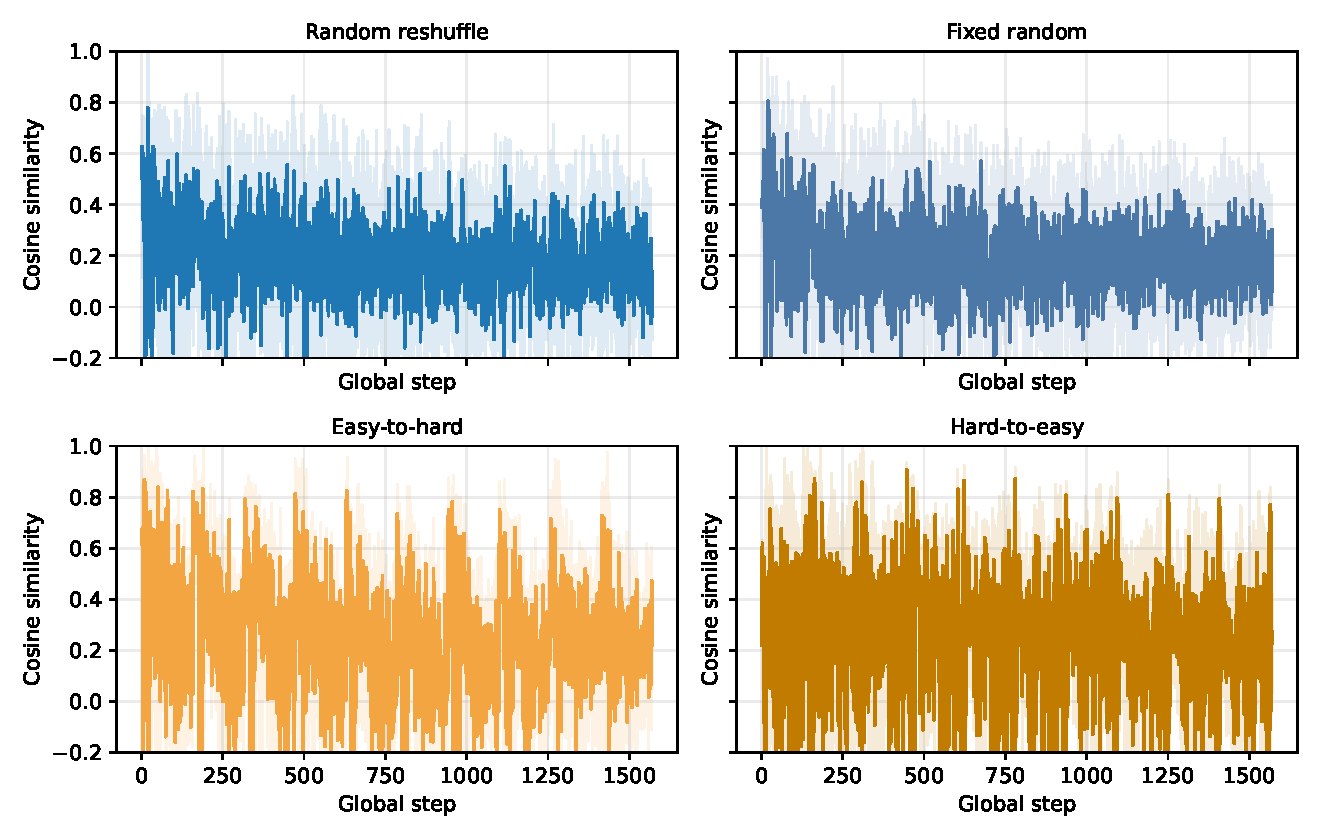
\includegraphics[width=0.95\textwidth]{results_v8/figures/stable_cosine_panels.pdf}
  \caption{Gradient cosine similarity for the four trainable orders, one
  panel per method. Shaded bands show one standard deviation across seeds.}
  \label{fig:app-cosine}
\end{figure*}

\begin{figure*}[!h]
  \centering
  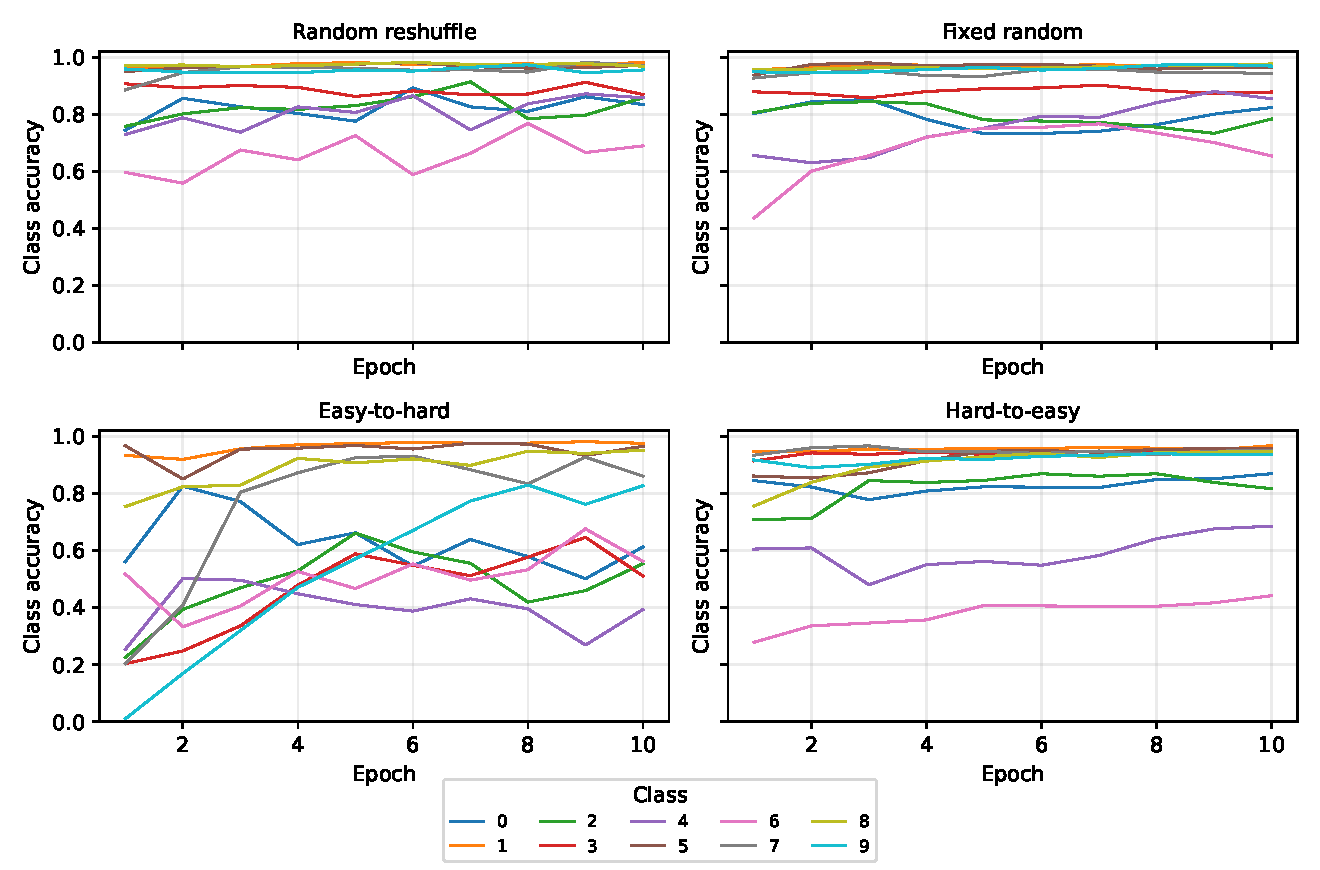
\includegraphics[width=0.95\textwidth]{results_v8/figures/stable_class_accuracy_curves.pdf}
  \caption{Class-wise accuracy evolution for the four trainable orders.
  The curricula remain finite but produce less balanced class behavior than
  the IID baselines.}
  \label{fig:app-classes}
\end{figure*}

\begin{figure}[!h]
  \centering
  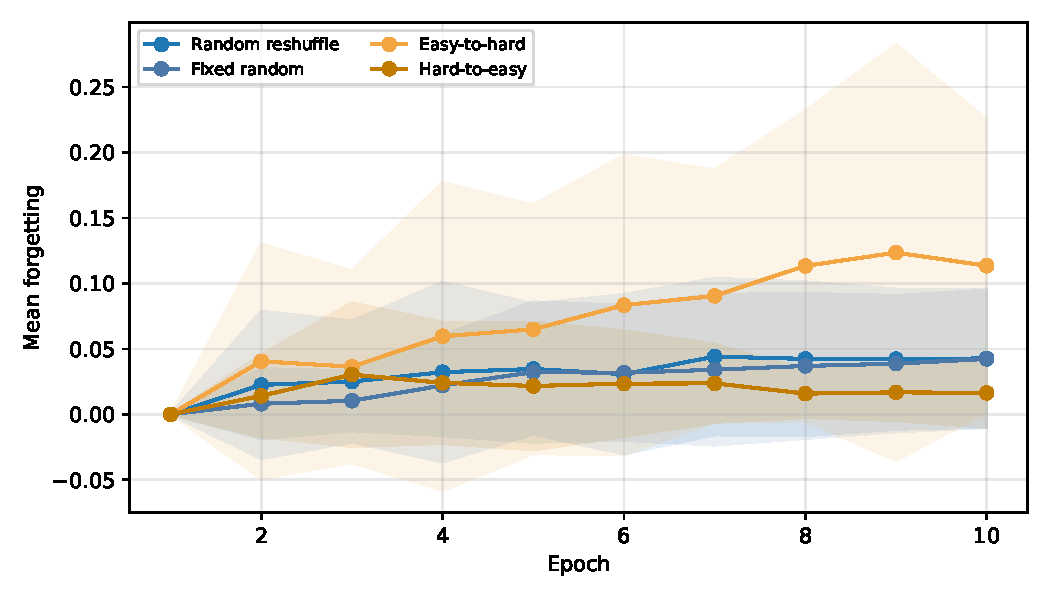
\includegraphics[width=\columnwidth]{results_v8/figures/stable_forgetting.pdf}
  \caption{Mean forgetting versus epoch for the four trainable orders.
  Easy-to-hard curriculum exhibits the largest retention gap.}
  \label{fig:app-forgetting}
\end{figure}

\begin{thebibliography}{1}
\providecommand{\newblock}{\relax}

\bibitem{bottou2018}
L.~Bottou, F.~E. Curtis, and J.~Nocedal, ``Optimization methods for large-scale
  machine learning,'' \emph{SIAM Review}, vol.~60, no.~2, pp. 223--311, 2018.

\bibitem{gurbuzbalaban2021}
M.~G{\"u}rb{\"u}zbalaban, A.~Ozdaglar, and P.~A. Parrilo, ``Why random
  reshuffling beats stochastic gradient descent,'' \emph{Mathematical
  Programming}, vol. 186, pp. 49--84, 2021.

\bibitem{bengio2009curriculum}
Y.~Bengio, J.~Louradour, R.~Collobert, and J.~Weston, ``Curriculum learning,''
  in \emph{Proceedings of the 26th International Conference on Machine
  Learning}, 2009, pp. 41--48.

\bibitem{loshchilov2019adamw}
I.~Loshchilov and F.~Hutter, ``Decoupled weight decay regularization,'' in
  \emph{International Conference on Learning Representations}, 2019.

\bibitem{xiao2017fashion}
H.~Xiao, K.~Rasul, and R.~Vollgraf, ``Fashion-mnist: A novel image dataset for
  benchmarking machine learning algorithms,'' \emph{arXiv preprint
  arXiv:1708.07747}, 2017.

\bibitem{mccloskey1989}
M.~McCloskey and N.~J. Cohen, ``Catastrophic interference in connectionist
  networks: The sequential learning problem,'' \emph{Psychology of Learning and
  Motivation}, vol.~24, pp. 109--165, 1989.

\end{thebibliography}

\end{document}
